\chapter{Dostosowanie Sirius Web dla systemu BalticLSC}

Z metamodelu EMF języka \gls{CAL} systemu \emph{BalticLSC}
opisanego w rozdziale~\ref{chapter:cal-metamodel} do tej pory korzystano w
\emph{Sirius Desktop}, w którym to został on przygotowany. W tym rozdziale
zostaną opisane kroki potrzebne do użycia go w \emph{Sirius Web}, aby otrzymać
aplikację przeglądarkową umożliwiającą edycję modeli języka \gls{CAL}.
Zostaną również omówione modyfikacje edytora \emph{Sirius Web}, które
zostały wykonane, aby poprawić jego integrację z systemem \emph{BalticLSC} oraz
umożliwić realizację walidacji semantycznej modelu.

\section{Użycie metamodelu języka CAL w Sirius Web}

Chcąc wykorzystać metamodel \gls{EMF} w \emph{Sirius Web} należy wskazać gdzie
on się znajduje oraz z jakich klas się składa, aby klasy te mogły zostać
dołączone do pliku \gls{JAR} serwera, a później odczytane przez moduły
\emph{Sirius
	Web} podczas uruchamiania aplikacji.

Dla \emph{Sirius Web} nie istnieje obecnie dokumentacja, co utrudnia jego
wykorzystanie z~własnym metamodelem. W serwisie GitHub istnieje repozytorium
\texttt{sirius-web}~\cite{sirius-web-github} zawierające kod~źródłowy aplikacji
przeglądarkowej
bazującej na \emph{Sirius Web}. Jest ona skonfigurowana do~wykorzystywania
metamodelu \emph{Sample Flow}~\cite{flow-network-github}
przygotowanego przez firmę \emph{Obeo Network}. Znajduje się on w innym
repozytorium (\texttt{Flow-Designer}~\cite{flow-network-github}) i jest
zwykłym metamodelem \gls{EMF}.
Należy więc wzorować się na tym przykładowym repozytorium w celu stworzenia
własnego edytora modeli.
W ramach tej pracy magisterskiej stworzono kopię repozytorium
\texttt{sirius-web} i skonfigurowano je, aby wykorzystywało metamodel
języka \gls{CAL} opisany w rozdziale~\ref{chapter:cal-metamodel}.

\emph{Sirius Web} do zarządzania projektem i wyrażania zależności między
pakietami wykorzystuje narzędzie \emph{Apache Maven}~\cite{maven-homepage}.
Aby wykorzystać klasy metamodelu \gls{EMF} w \emph{Sirius Web}
należy do katalogów wygenerowanych przez \emph{Sirius Desktop} dodać pliki
\gls{POM} (\texttt{pom.xml}), które zawierają informacje o nazwie projektu i
jego
zależnościach. Wygenerowane projekty metamodelu \gls{EMF} to projekty
\emph{Eclipse}.
Oznacza to, że zależności projektów,
na~które składa się całość metamodelu są zapisane w plikach
\texttt{MANIFEST.MF}, a pozostałe informacje o~projekcie znajdują się w
plikach \texttt{build.properties}, \texttt{plugin.properties} oraz
\texttt{plugin.xml}. Te pliki nie są wykrywane domyślnie przez \emph{Maven},
więc
próba wykorzystania takiego projektu zakończy się błędem. Aby wykorzystać je w
\emph{Sirius Web} należy odpowiednio skonfigurować ich pliki
\gls{POM}~\cite{maven-tycho-tutorial}.

Po pierwsze należy do listy repozytoriów pakietów dodać repozytorium
\emph{Eclipse} w formacie \texttt{p2}. Jest to format wykorzystywany przez
projekty \emph{Eclipse}, podczas gdy \emph{Maven} wykorzystuje repozytoria w
swoim własnym formacie. Fragment pliku \texttt{pom.xml} konfigurujący to
repozytorium znajduje się na listingu~\ref{lst:pom-eclipse-repository}.

\begin{lstlisting}[language=XML,
    caption={Konfiguracja repozytorium \emph{Eclipse} w \texttt{pom.xml}.},
    label={lst:pom-eclipse-repository}]
<repositories>
  <repository>
    <id>eclipse</id>
    <layout>p2</layout>
    <url>http://download.eclipse.org/releases/2021-09</url>
  </repository>
</repositories>
\end{lstlisting}

Kolejno w plikach \texttt{pom.xml} projektów metamodelu \gls{EMF} należy
zdefiniować, że~są~to~projekty \emph{Eclipse}, poprzez dodanie elementu
\texttt{packaging} z wartością \texttt{eclipse-plugin}. Zostało
to~zademonstrowane na listingu~\ref{lst:pom-packaging} w linii 9.

\begin{lstlisting}[language=XML,
    caption={Plik \texttt{pom.xml} dla jednego z projektów metamodelu
      \gls{EMF}.},
    label={lst:pom-packaging}]
<?xml version="1.0" encoding="UTF-8" ?>
<project
  xmlns="http://maven.apache.org/POM/4.0.0"
  xmlns:xsi="http://www.w3.org/2001/XMLSchema-instance"
  xsi:schemaLocation="http://maven.apache.org/POM/4.0.0 http://maven.apache.org/xsd/maven-4.0.0.xsd"
>
  <modelVersion>4.0.0</modelVersion>
  <artifactId>eu.balticlsc.model.CAL</artifactId>
  <packaging>eclipse-plugin</packaging>

  <parent>
    <groupId>eu.balticlsc.model</groupId>
    <artifactId>model</artifactId>
    <version>0.1.0-SNAPSHOT</version>
  </parent>
</project>
\end{lstlisting}

Następnie w sekcji \texttt{build} pliku \texttt{pom.xml} należy dodać pluginy
\emph{Maven Tycho}~\cite{maven-tycho-homepage}. Jest~to~zestaw rozszerzeń do
\emph{Apache Maven}
pozwalający na wykorzystanie projektów \emph{Eclipse}. Fragment
wymaganej konfiguracji znajduje się na
listingu~\ref{lst:pom-maven-tycho-plugins}. Ważne jest, aby wskazać konkretną
wersję środowiska uruchomieniowego języka Java. W tym przypadku jest to Java
11. Jest to jedyna wersja oficjalnie obsługiwana przez \emph{Sirius Web}.
Inne wersje nie są wspierane.

\begin{lstlisting}[language=XML,
    caption={Konfiguracja rozszerzeń \emph{Maven Tycho} w \texttt{pom.xml}.},
    label={lst:pom-maven-tycho-plugins}]
<build>
  <plugins>
    <plugin>
      <groupId>org.eclipse.tycho</groupId>
      <artifactId>tycho-maven-plugin</artifactId>
      <version>2.5.0</version>
      <extensions>true</extensions>
    </plugin>

    <plugin>
      <groupId>org.eclipse.tycho</groupId>
        <artifactId>tycho-packaging-plugin</artifactId>
         <version>2.5.0</version>
         <executions>
          <execution>
            <phase>package</phase>
            <id>package-feature</id>
              <configuration>
                <finalName>${project.artifactId}_${unqualifiedVersion}.${buildQualifier}</finalName>
              </configuration>
        </execution>
      </executions>
    </plugin>

    <plugin>
      <groupId>org.eclipse.tycho</groupId>
      <artifactId>target-platform-configuration</artifactId>
      <version>2.5.0</version>

      <configuration>
        <executionEnvironment>JavaSE-11</executionEnvironment>

        <!-- ... konfiguracja platformy -->
      </configuration>
    </plugin>
  </plugins>
</build>
\end{lstlisting}

Tak przygotowany projekt \emph{Maven} będzie wykrywał zależności zdefiniowane w
odpowiednich plikach \emph{Eclipse} i będzie możliwy do wykorzystania jako
zależność w innych projektach \emph{Maven}. Można to potwierdzić uruchamiając
komendę \lstinline{mvn clean verify}. Model można teraz dodać do pliku
\texttt{pom.xml} aplikacji serwerowej \emph{Sirius Web} (projekt
\texttt{sirius-web-sample-application}) dodając odwołania do 3 pakietów:
głównego pakietu modelu, pakietu \texttt{.edit} oraz pakietu \texttt{.design}.
Odwołania te widoczne są na listingu~\ref{lst:pom-metamodel-dependencies}.

\begin{lstlisting}[language=XML,
    caption={Odwołania do pakietów metamodelu w \texttt{pom.xml} aplikacji
    serwerowej \emph{Sirius Web}},
    label={lst:pom-metamodel-dependencies}]
<dependency>
  <groupId>eu.balticlsc.model</groupId>
  <artifactId>eu.balticlsc.model.CAL</artifactId>
  <version>0.1.0-SNAPSHOT</version>
</dependency>
<dependency>
  <groupId>eu.balticlsc.model</groupId>
  <artifactId>eu.balticlsc.model.CAL.edit</artifactId>
  <version>0.1.0-SNAPSHOT</version>
</dependency>
<dependency>
  <groupId>eu.balticlsc.model</groupId>
  <artifactId>eu.balticlsc.model.CAL.design</artifactId>
  <version>0.1.0-SNAPSHOT</version>
</dependency>
\end{lstlisting}

Taka konfiguracja zależności między projektami pozwala na wykorzystanie klas
metamodelu w kodzie źródłowym \emph{Sirius Web}. Należy teraz w klasie
\texttt{SampleEMFConfiguration} zarejestrować klasy
odpowiedzialne za metamodel: \texttt{EPackage} oraz \texttt{AdapterFactory}.
Fragment kodu realizujący to jest znajduje się na
listingu~\ref{lst:registering-emf-classes}. Później w klasie
\texttt{SampleSiriusConfiguration} należy wskazać ścieżkę do pliku
\texttt{*.odesign} metamodelu znajdującego się w pakiecie \texttt{.design}.
Odpowiedni fragment znajduje się na
listingu~\ref{lst:registering-odesign-path}.

\begin{lstlisting}[language=Java,
    caption={Rejestracja klas przygotowanego metamodelu EMF w klasie
    \texttt{SampleEMFConfiguration}.},
    label={lst:registering-emf-classes}]
    @Bean
    public AdapterFactory calAdapterFactory() {
        return new CALItemProviderAdapterFactory();
    }

    @Bean
    public EPackage calEPackage() {
        return CALPackage.eINSTANCE;
    }
\end{lstlisting}

\begin{lstlisting}[language=Java,
    caption={Wskazanie ścieżki do pliku \texttt{*.odesign} w klasie
    \texttt{SampleSiriusConfiguration}.},
    label={lst:registering-odesign-path}]
    @Override
    public List<String> getODesignPaths() {
        return List.of("description/CAL.odesign"); //$NON-NLS-1$
    }
\end{lstlisting}

Po tych modyfikacjach w aplikacji \emph{Sirius Web} można tworzyć i edytować
modele nowo stworzonego metamodelu \gls{EMF}. Zrzut ekranu z aplikacji
przeglądarkowej widoczny jest
na~rysunku~\ref{rys:sirius-web-base-metamodel-model}.

% \begin{noindent}
\begin{figure}[!hb]
  \centering

  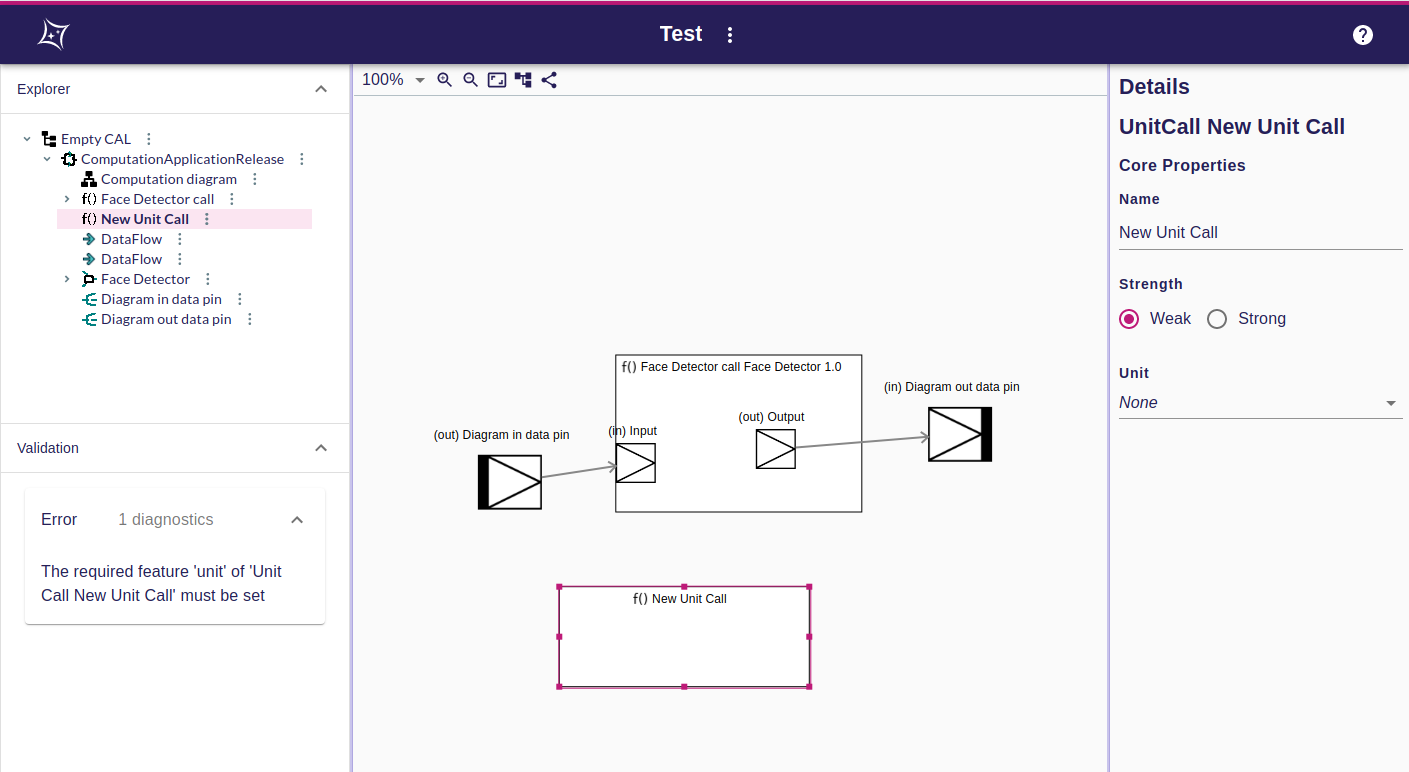
\includegraphics[width=0.95\linewidth]{./images/sirius-web-base-metamodel-model.png}
  \caption{Edycja modelu bazującego na przygotowanym metamodelu EMF w
  \emph{Sirius Web}.}\label{rys:sirius-web-base-metamodel-model}
\end{figure}
% \end{noindent}

W \emph{Sirius Web} można zdefiniować szablony modeli, które użytkownik może
wykorzystać chcąc stworzyć nowy model w projekcie. Umożliwia to prostszy
sposób na stworzenie chociażby pustego modelu, ponieważ przycisk tworzenia
modelu
na podstawie szablonu jest bardziej wyeksponowany w interfejsie użytkownika niż
przyciski tworzenia modelu z drzewa elementów projektu po lewej stronie.
Aby dodać nowy szablon należy dodać nowy opis \emph{stereotypu} w metodzie
\texttt{addStereotypeDescriptions} klasy
\texttt{StereotypeDescriptionRegistryConfigurer}. Kod odpowiedzialny za dodanie
nowego pustego szablonu modelu został przedstawiony
na~listingu~\ref{lst:empty-cal-model-template}. Interfejs użytkownika aplikacji
\emph{Sirius Web} wyświetlający nowo dodany szablon pustego modelu języka
\gls{CAL} został przedstawiony na
rysunku~\ref{rys:sirius-web-new-model-template}.

\begin{lstlisting}[float,
    floatplacement=!hb,
    language=Java,
    caption={Dodanie nowego pustego szablonu modelu języka CAL.},
    label={lst:empty-cal-model-template}]
    @Override
    public void addStereotypeDescriptions(IStereotypeDescriptionRegistry registry) {
        registry.add(new StereotypeDescription(
          UUID.nameUUIDFromBytes("empty_cal".getBytes()), //$NON-NLS-1$
          "Empty CAL", //$NON-NLS-1$
          this::getEmptyCALContent
        ));
    }

    private String getEmptyCALContent() {
        return this.stereotypeBuilder.getStereotypeBody(
          CALFactory.eINSTANCE.createComputationApplicationRelease()
        );
    }
\end{lstlisting}

% \begin{noindent}
\begin{figure}[!hb]
  \centering

  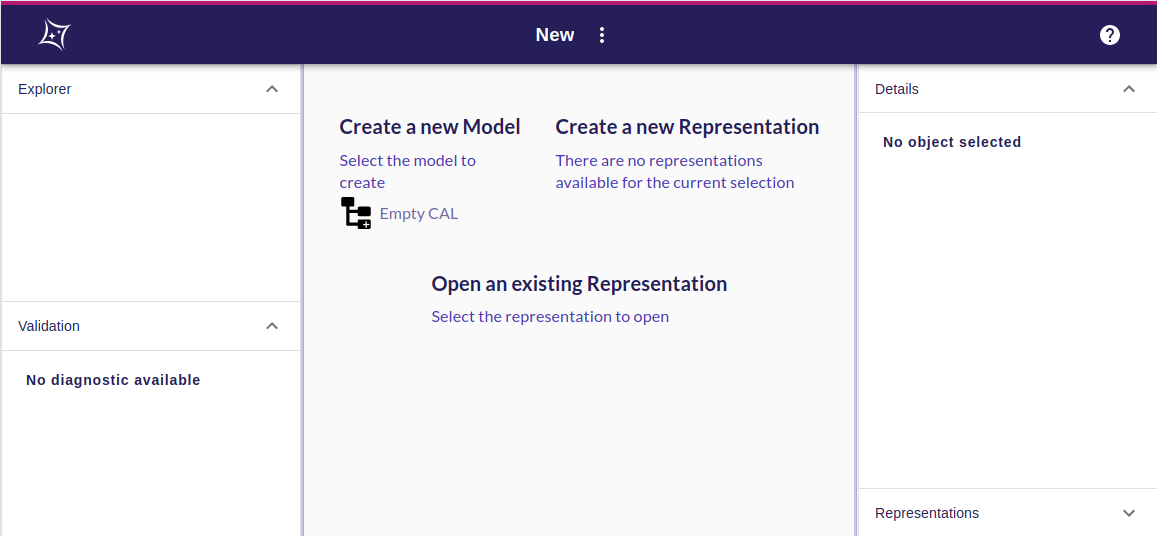
\includegraphics[width=0.95\linewidth]{./images/sirius-web-new-model-template.png}
  \caption{Szablon nowego pustego modelu języka
    \gls{CAL} w \emph{Sirius Web}.}\label{rys:sirius-web-new-model-template}
\end{figure}
% \end{noindent}

\subsection{Uruchamianie testów metamodelu za pomocą Maven}

W sekcji~\ref{sec:testy-metamodelu} opisano testy zmodyfikowanego zachowania
metamodelu EMF\@. Były one~uruchamianie w \emph{Sirius Desktop}. Z uwagi na
fakt, że
wygenerowany projekt z testami jest projektem typu \emph{Eclipse}, \emph{Apache
	Maven} nie ma możliwości wykonania tych testów podczas standardowego
polecenia
wykonania testów \lstinline{mvn test}.

Z pomocą przychodzi tutaj zestaw narzędzi \emph{Maven Tycho} wykorzystany do
połączenia metamodelu \gls{EMF} z \emph{Sirius Web}. Zawiera on rozszerzenie
\texttt{tycho-surefire-plugin}~\cite{maven-surefire-plugin-homepage}, które w
trakcie fazy wykonywania testów
integracyjnych w \emph{Maven} wykonuje również testy metamodelu zdefiniowane w
\emph{JUnit} i opisane w sekcji~\ref{sec:testy-metamodelu}.
Wykorzystanie go w pliku \texttt{pom.xml} projektu z testami (folder
\texttt{.tests}) przedstawione jest na
listingu~\ref{lst:pom-maven-surefire-plugin}. Należy w nim wskazać gdzie
znajduje się kod źródłowy testów oraz ścieżkę do pakietu z testami, a także
nazwę klasy grupującej wszystkie testy.

\begin{lstlisting}[float,
    floatplacement=!hb,
    language=XML,
    caption={Wykorzystanie rozszerzenia \emph{Maven Surefire} w
    \texttt{pom.xml} projektu z testami metamodelu.},
    label={lst:pom-maven-surefire-plugin}]
<build>
  <testSourceDirectory>${project.basedir}/src</testSourceDirectory>
  <plugins>
    <plugin>
      <groupId>org.eclipse.tycho</groupId>
      <artifactId>tycho-surefire-plugin</artifactId>
      <configuration>
        <testSuite>eu.balticlsc.model.CAL.tests</testSuite>
        <testClass>eu.balticlsc.model.CAL.tests.CALAllTests</testClass>
      </configuration>
      <version>2.5.0</version>
    </plugin>
  </plugins>
</build>
\end{lstlisting}

Po tak zmodyfikowanej konfiguracji
testy metamodelu \gls{EMF} w \emph{Maven} można uruchomić komendą
\lstinline{mvn verify}. Są one uruchamiane w fazie testów integracyjnych
(\texttt{verify}), a
więc po fazie budowania aplikacji (\texttt{package}). Powoduje to, że
uruchomienie testów metamodelu za~pomoca \emph{Maven} trwa dłużej (około
18 sekund), niż
wewnątrz \emph{Sirius Desktop} (mniej niż~1~sekunda), ponieważ projekt
najpierw musi zostać zbudowany. Dodatkowy narzut czasowy wprowadza także
komunikacja
\emph{Maven} z repozytorium \emph{Eclipse}, z którego pobierane są pakiety.
Niemniej jednak możliwość uruchomienia testów metamodelu w \emph{Maven} pozwala
na~uruchomienie ich z linii wiersza poleceń bez uruchamiania \emph{Sirius
	Desktop}, co przydaje się~w~środowisku serwerowym.

\section{Integracja przybornika BalticLSC w Sirius Web}

Edytor diagramów dostępny w aplikacji przeglądarkowej platformy
\emph{BalticLSC}
umożliwia dodawanie wywołań modułów obliczeniowych do diagramu za pomocą
przybornika (ang.~\emph{\selectlanguage{english}toolbox}). Użytkownik
przeglądający bibliotekę dostępnych modułów
obliczeniowych może dodać wybrane z nich do przybornika. Zrzut ekranu
biblioteki modułów z kilkoma modułami dodanymi do~przybornika jest widoczny na
rysunku~\ref{rys:balticlsc-development-shelf}. W trakcie edycji
diagramu ikony dodanych do~przybornika modułów są widoczne z lewej strony
diagramu (rysunek~\ref{rys:balticlsc-diagram-toolbox}). Kliknięcie przycisku
jednego z modułów zaznacza go, po
czym kliknięcie na diagram dodaje moduł w określonym miejscu. Stan
po dodaniu wywołania modułu obliczeniowego wybranego
na~rysunku~\ref{rys:balticlsc-diagram-toolbox} jest widoczny na
rysunku~\ref{rys:balticlsc-after-adding-unit-call}.

% \begin{noindent}
\begin{figure}[!hb]
  \centering

  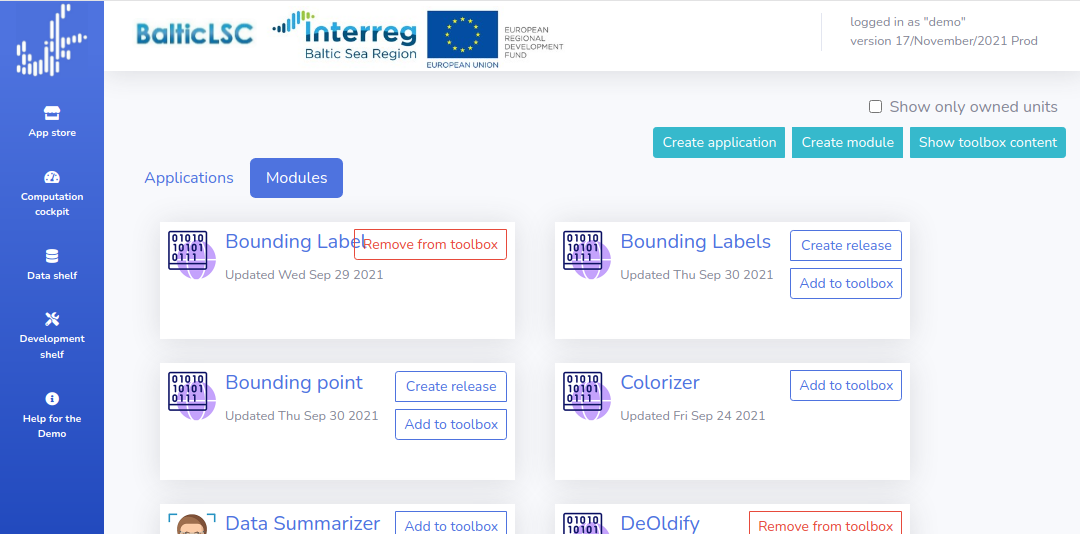
\includegraphics[width=0.95\linewidth]{./images/balticlsc-development-shelf.png}
  \caption{Biblioteka modułów obliczeniowych platformy
  \emph{BalticLSC}.}\label{rys:balticlsc-development-shelf}
\end{figure}
% \end{noindent}

% \begin{noindent}
\begin{figure}[!hb]
  \centering

  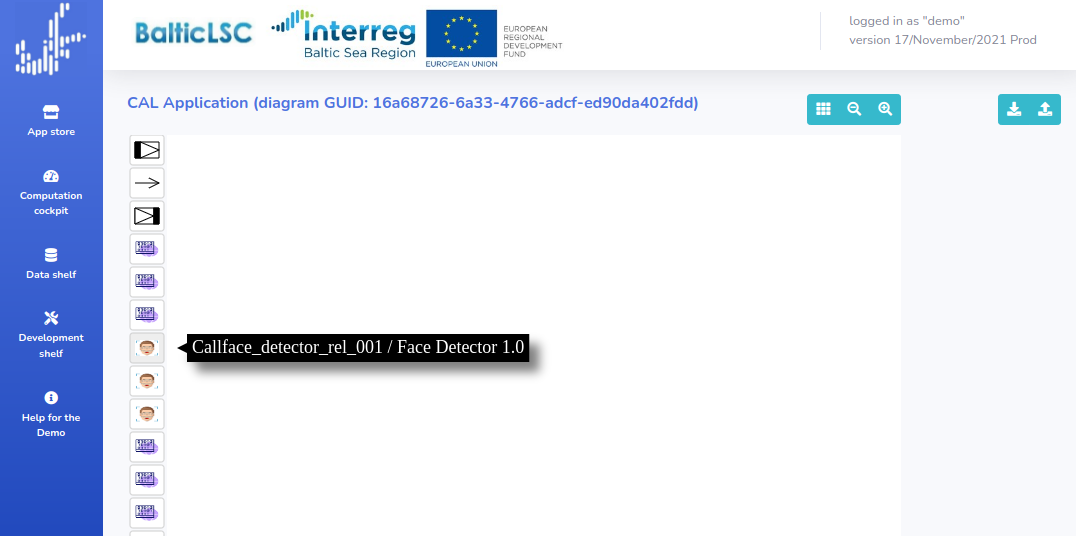
\includegraphics[width=0.95\linewidth]{./images/balticlsc-diagram-toolbox.png}
  \caption{Przybornik dostępny w edytorze diagramów platformy
  \emph{BalticLSC}.}\label{rys:balticlsc-diagram-toolbox}
\end{figure}
% \end{noindent}

% \begin{noindent}
\begin{figure}[!hb]
  \centering

  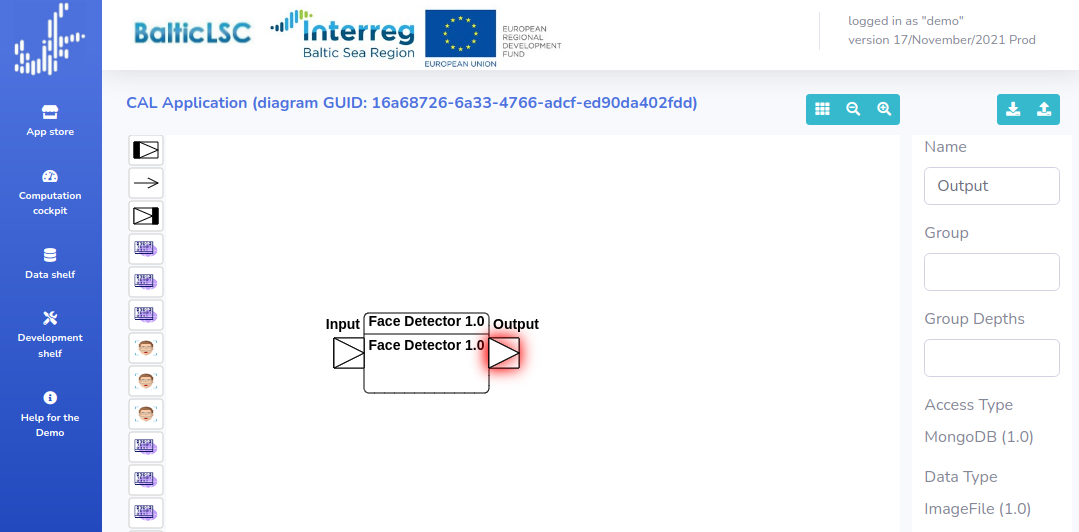
\includegraphics[width=0.95\linewidth]{./images/balticlsc-after-adding-unit-call.png}
  \caption{Edytor diagramów \emph{BalticLSC} po dodaniu modułu obliczeniowego z
  przybornika.}\label{rys:balticlsc-after-adding-unit-call}
\end{figure}
% \end{noindent}

Rozwiązanie przybornika pozwala użytkownikowi podzielić proces pracy z modułami
obliczeniowymi na 2 etapy: wybór interesujących modułów z listy potencjalnie
tysięcy dostępnych modułów obliczeniowych, a później użycie
wybranego podzbioru modułów na~diagramach.

W edytorze diagramów z \emph{Sirius Web} domyślnie nie ma przybornika ani
integracji z~zewnętrznymi serwisami w celu pobrania listy modułów
obliczeniowych. Definicje wszystkich modułów obliczeniowych, które mają być
dostępne w modelu muszą być zdefiniowane jako
elementy modelu (\texttt{ComputationUnitRelease}). Mechanizmy dostępne w
metamodelu \gls{EMF} nie pozwalają na komunikację z zewnętrznymi serwisami,
więc pobieranie danych o modułach obliczeniowych znajdujących się w przyborniku
danego użytkownika musi zostać zrealizowane na poziomie \emph{Sirius Web}.
Ponadto, skoro ma być pobrana zawartość przybornika konkretnego użytkownika,
aplikacja \emph{Sirius Web} musi znać jego informacje uwierzytelniające, aby
móc je~dołączyć wysyłając zapytanie \gls{API} do serwera \emph{BalticLSC}.
Szczegóły odtworzenia
mechanizmu przybornika w \emph{Sirius Web} oraz jego integracja z
\emph{BalticLSC} zostały opisane w kolejnych sekcjach.

\subsection{Pobranie zawartości
	przybornika}\label{sec:pobranie-zawartosci-przybornika}

Serwer aplikacyjny \emph{BalticLSC} udostępnia interfejs \gls{API} w formacie
\gls{REST}, który jest używany do komunikacji z aplikacją przeglądarkową tego
serwisu. Ten interfejs można również wykorzystać w \emph{Sirius Web} aby pobrać
zawartość przybornika. W tym celu należy wysłać uwierzytelnione zapytanie
protokołu \gls{HTTP} pytając o zasób \texttt{/backend/dev/toolbox/}. W
odpowiedzi zwrócona jest lista składająca się z~informacji o wybranych modułach
obliczeniowych. Zawiera ona wszystkie detale potrzebne do utworzenia obiektu
modułu obliczeniowego (\texttt{ComputationUnitRelease}) oraz jego wywołania
(\texttt{UnitCall}) w modelu, łącznie z informacjami o zadeklarowanych portach
tego modułu.

Należałoby więc z aplikacji przeglądarkowej \emph{Sirius Web} wysłać takie
zapytanie do serwera \emph{BalticLSC}, a następnie wyświetlić otrzymane moduły
obliczeniowe na ekranie. Już na samym etapie wysyłania zapytania do serwera
\emph{BalticLSC} pojawiają się dwa problemy.

Pierwszym problemem jest sposób uwierzytelniania użytkownika. Zawartość
przybornika jest powiązana z konkrenym kontem użytkownika w systemie
\emph{BalticLSC}. Wysyłając więc zapytanie o przybornik należy dodatkowo
załączyć w nagłówku \gls{HTTP} \texttt{Authorization}
token uwierzytelniający w formacie \gls{JWT}. W tokenie tym znajdują się
informacje o nazwie użytkownika, do którego należy token (pole \texttt{sub}
oraz \texttt{unique\_name}). Zawartość pola z
danymi tokena widoczna jest na listingu~\ref{lst:balticlsc-jwt-payload}.
Ponadto, każdy token \gls{JWT} posiada podpis weryfikujący jego prawdziwość.
Służy on potwierdzeniu, że token został przygotowany przez serwis
\emph{BalticLSC} w drodze poprawnego logowania do serwisu, a nie został
wytworzony przez osobę próbującą podszyć się pod danego użytkownika.

\begin{lstlisting}[float,
    floatplacement=hb,
    language=java,
    caption={Zawartość pola z danymi w tokenie \gls{JWT} z serwisu
      \emph{BalticLSC}.},
    label={lst:balticlsc-jwt-payload}]
{
  "unique_name": "demo",
  "sub": "demo",
  "jti": "bcbbbbe299424a60a3dd4cb918a1364c",
  "sid": "37a970ff48db49e6a5e4c4bb5912d4b4",
  "exp": 1641671342,
  "iss": "wut.balticlsc.eu",
  "aud": "wut.balticlsc.eu"
}
\end{lstlisting}

W pracy magisterskiej założono, że token \gls{JWT} zostanie dostarczony do
edytora diagramów z zewnętrznego źródła. W przypadku wykorzystania edytora
diagramów \emph{Sirius Web} w innej aplikacji przeglądarkowej, to właśnie ta
zewnętrzna aplikacja przeglądarkowa dostarczy informacje o tokenie \gls{JWT}
podczas wywoływania funkcji rozpoczynającej wyświetlanie diagramu. Zostało to
opisane szczegółowo w sekcji~\ref{sec:uzycie-sirius-web-w-balcitlsc}.

Podczas pracy z pełnym pełnym interfejsem \emph{Sirius Web} (a nie tylko samym
edytorem diagramów) został dostarczony przycisk otwierający okno
dialogowe, w którym użytkownik może wprowadzić swój token \gls{JWT}. Znajdują
się w nim także instrukcje jak taki token pozyskać. Ponieważ jest to złożony
proces, który wymaga otworzenia narzędzi programistycznych przeglądarki, został
dostarczony przycisk \emph{\selectlanguage{english}GET DEMO USER TOKEN}, który
pozwala pobrać token użytkownika demonstracyjnego \emph{BalticLSC}.
Wysyła on zapytanie z prośbą o zalogowanie użytkownika demonstracyjnego,
którego dane logowania są publiczne dostępne, a następnie otrzymany token
uwierzytelniający wprowadza do pola widocznego w oknie dialogowym. W~ten~sposób
można w łatwy sposób otrzymać poprawny token i rozpocząć działanie z
\emph{Sirius Web} wykorzystując przybornik użytkownika demonstracyjnego.
Zrzut ekranu przedstawiający okno dialogowe pozwalające wprowadzić token
\gls{JWT} użytkownika jest widoczne na
rysunku~\ref{rys:balticlsc-change-jwt-modal}.

% \begin{noindent}
\begin{figure}[!hb]
  \centering

  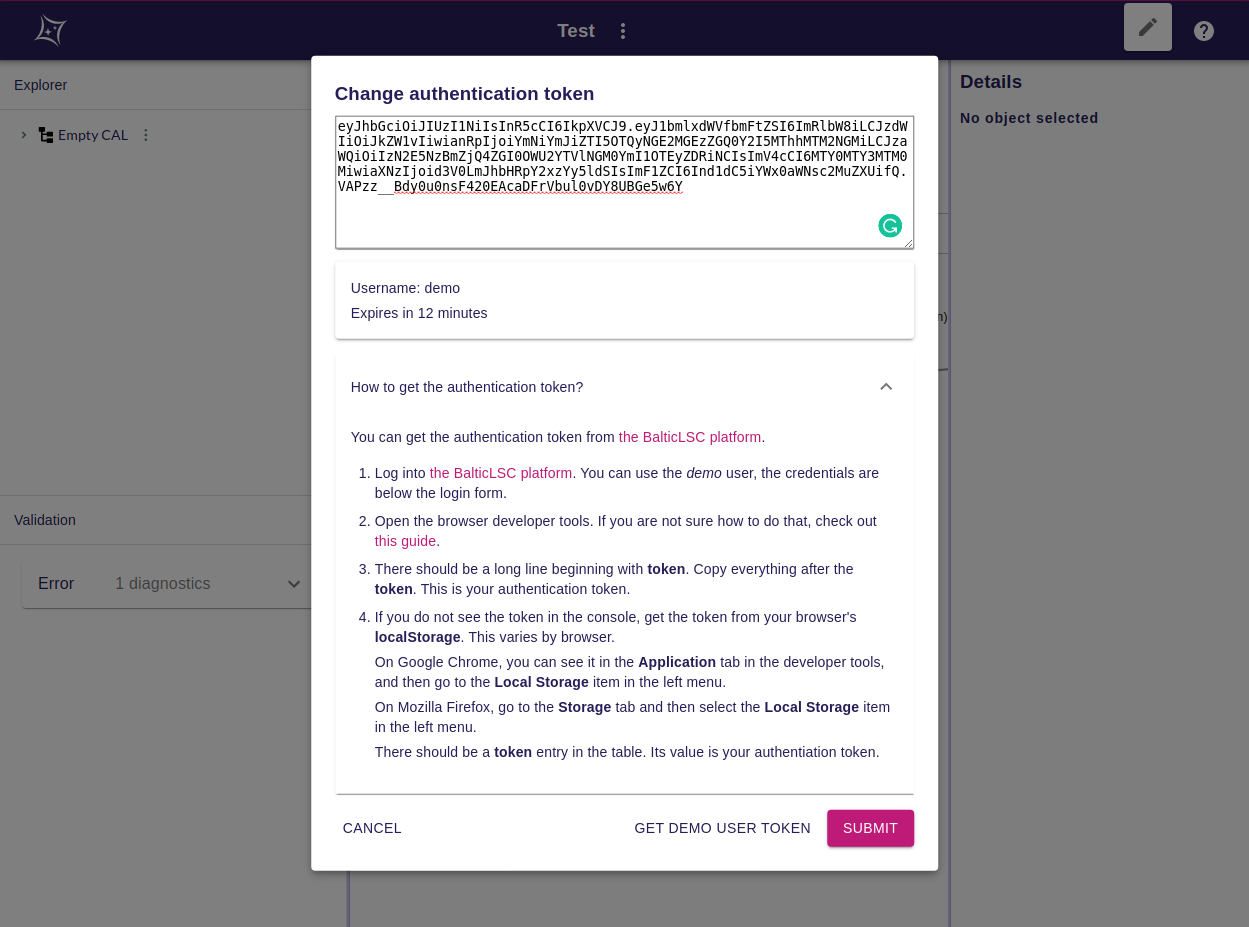
\includegraphics[width=0.95\linewidth]{./images/balticlsc-change-jwt-modal-with-instructions.png}
  \caption{Okno dialogowe do wprowadzenia tokenu \gls{JWT}
    użytkownika.}\label{rys:balticlsc-change-jwt-modal}
\end{figure}
% \end{noindent}

Drugim z problemów występujących podczas komunikacji z \gls{API}
\emph{BalticLSC} jest mechanizm \gls{CORS}~\cite{cors-documentation}. Aktywuje
się on ponieważ serwer
aplikacyjny \emph{BalticLSC} oraz aplikacja przeglądarkowa \emph{Sirius Web} są
uruchomione na różnych adresach w sieci Internet. Odpowiedzi z serwera
aplikacyjnego \emph{BalticLSC} nie zawierają odpowiednich nagłówków \gls{HTTP}
związanych z \gls{CORS},
więc przeglądarka blokuje połączenia do tego serwera podczas próby ich wysłania
ze
strony internetowej zawierającej \emph{Sirius Web}. W~przypadku edytora
diagramów dostarczonego z \emph{BalticLSC} \gls{CORS} nie występuje, ponieważ
edytor diagramów oraz serwer znajdują się pod tym samym adresem internetowym
\url{https://balticlsc.iem.pw.edu.pl/}, więc przeglądarka zezwala na te
połączenia bez wymogu dodatkowych nagłówków w odpowiedziach z serwera.

Rozwiązaniem na problem braku nagłówków \gls{CORS} w odpowiedziach z serwera
\emph{BalticLSC} jest wykorzystanie innego serwera jako pośredniczącego w ruchu
między aplikacją przeglądarkową \emph{Sirius Web}, a serwerem \emph{BalticLSC}
(ang. \emph{\selectlanguage{english}proxy}). Schemat komunikacji między
aplikacją \emph{Sirius Web} uruchomioną w przeglądarce a serwerem
\emph{BalticLSC} z wykorzystaniem serwera pośredniczącego przedstawiono na
rysunku~\ref{rys:balticlsc-proxy-sequence-diagram}.

% \begin{noindent}
\begin{figure}[!hb]
  \centering

  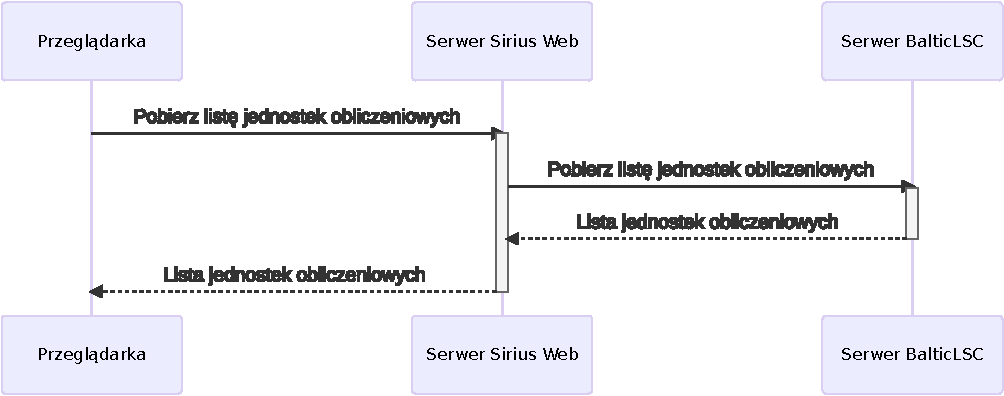
\includegraphics[width=0.95\linewidth]{./images/balticlsc-proxy-sequence-diagram.pdf}
  \caption{Diagram sekwencji pobierania listy modułów obliczeniowych z
    wykorzystaniem serwera pośredniczącego.}\label{rys:balticlsc-proxy-sequence-diagram}
\end{figure}
% \end{noindent}

% Kod źródłowy diagramu (Mermaid)
% https://mermaid-js.github.io/mermaid-live-editor/edit/#eyJjb2RlIjoic2VxdWVuY2VEaWFncmFtXG5wYXJ0aWNpcGFudCBicm93c2VyIGFzIFByemVnbMSFZGFya2FcbnBhcnRpY2lwYW50IHByb3h5IGFzIFNlcndlciBTaXJpdXMgV2ViXG5wYXJ0aWNpcGFudCBiYWx0aWNsc2MgYXMgU2Vyd2VyIEJhbHRpY0xTQ1xuXG5icm93c2VyIC0-PisgcHJveHk6IFBvYmllcnogbGlzdMSZIG1vZHXFgsOzdyBvYmxpY3plbmlvd3ljaFxucHJveHkgLT4-KyBiYWx0aWNsc2M6IFBvYmllcnogbGlzdMSZIG1vZHXFgsOzdyBvYmxpY3plbmlvd3ljaFxuXG5iYWx0aWNsc2MgLS0-Pi0gcHJveHk6IExpc3RhIG1vZHXFgsOzdyBvYmxpY3plbmlvd3ljaFxucHJveHkgLS0-Pi0gYnJvd3NlcjogTGlzdGEgbW9kdcWCw7N3IG9ibGljemVuaW93eWNoXG4iLCJtZXJtYWlkIjoie1xuICBcInRoZW1lXCI6IFwiZGVmYXVsdFwiXG59IiwidXBkYXRlRWRpdG9yIjpmYWxzZSwiYXV0b1N5bmMiOnRydWUsInVwZGF0ZURpYWdyYW0iOmZhbHNlfQ
%
% sequenceDiagram
% participant browser as Przeglądarka
% participant proxy as Serwer Sirius Web
% participant balticlsc as Serwer BalticLSC
%
% browser ->>+ proxy: Pobierz listę modułów obliczeniowych
% proxy ->>+ balticlsc: Pobierz listę modułów obliczeniowych
%
% balticlsc -->>- proxy: Lista modułów obliczeniowych
% proxy -->>- browser: Lista modułów obliczeniowych

Serwerem pośredniczącym może być na przykład serwer aplikacyjny \emph{Sirius
	Web}. Dodano do niego odpowiedni mechanizm tak, aby wszystkie zapytania
których adres
zaczyna się~od~\texttt{/balticlsc-proxy} przesyłane były do serwera
\emph{BalticLSC}, a odpowiedzi z serwera zwracane do~oryginalnego nadawcy
zapytania.

W przypadku uruchomienia edytora diagramów \emph{Sirius Web} jako część głównej
aplikacji przeglądarkowej \emph{BalticLSC} pod tym samym adresem co serwer
aplikacyjny tej platformy można zrezygnować z komunikacji z wykorzystaniem
serwera pośredniczącego i wysyłać zapytania bezpośrednio do serwera
aplikacyjnego \emph{BalticLSC}. W tej sytuacji mechanizm \gls{CORS} nie będzie
wykorzystany i przeglądarka pozwoli na wykonanie połączenia.

\subsection{Wyświetlenie zawartości przybornika w Sirius Web}

W sekcji~\ref{sec:pobranie-zawartosci-przybornika} opisany został mechanizm, za
pomocą którego aplikacja przeglądarkowa \emph{Sirius Web} ma dostęp do listy
modułów obliczeniowych dodanych do przybornika danego użytkownika. Zawartość
przybornika należy wyświetlić na ekranie w obrębie edytora diagramów, aby
użytkownik mógł z niego skorzystać. Realizacja tej funkcjonalności wymaga
modyfikacji interfejsu użytkownika \emph{Sirius Web}.

Warstwa interfejsu użytkownika \emph{Sirius Web} napisana jest w języku
\emph{TypeScript}~\cite{typescript-homepage}, który jest rozszerzeniem języka
\emph{JavaScript} dodającym
statyczne typowanie zmiennych. Kod~wykorzystuje bibliotekę
\emph{React}~\cite{react-homepage} do podziału warstwy wizualnej na mniejsze
komponenty i ich wyświetlenie. Podstawowe komponenty, z których można zbudować
edytor modeli bazujący na serwerze aplikacyjnym \emph{Sirius Web} są
zlokalizowane i udostępnione w repozytorium \texttt{sirius-components}.
W repozytorium \texttt{sirius-web} są one wykorzystane do zbudowania
przykładowej aplikacji przeglądarkowej do edycji modeli.
Jest ona demonstracją jak można ich użyć i może zostać dostosowana do własnych
potrzeb.

Zdecydowano, że w domyślnym interfejsie użytkownika aplikacji \emph{Sirius Web}
zaprezentowanym na rysunku~\ref{rys:sirius-web-base-metamodel-model}
odpowiednie miejsce na wyświetlenie przybornika znajduje się~nad~diagramem,
powyżej paska narzędzi, a poniżej górnej ciemnoniebieskiej belki z tytułem
projektu. Komponent \texttt{Workbench} odpowiedzialny za wyświetlenie edytora
diagramów (całość
interfejsu \emph{Sirius Web} oprócz górnej ciemnoniebieskiej belki) nie
ma możliwości pokazania dodatkowych komponentów zdefiniowanych przez
programistę pracującego nad własnym edytorem diagramów. Wyświetla on zawsze
komponenty w ustalonym porządku:

\begin{itemize}
	\item Panel z lewej strony składający się z drzewa elementów projektu na górze oraz informacji diagnostycznych modelu na dole.
	\item Panel główny z edytorem aktualnie wybranego diagramu. Gdy żaden nie jest wybrany, wyświetlone są tam przyciski umożliwiające łatwe stworzenie pierwszego modelu w~projekcie.
	\item Panel z prawej strony składający się z detali aktualnie wybranego elementu diagramu.
\end{itemize}

Chcąc dodać nowy element interfejsu użytkownika wymagane jest skopiowanie kodu
źródłowego komponentu \texttt{Workbench} z repozytorium
\texttt{sirius-components} do własnej kopii repozytorium \texttt{sirius-web} i
skorzystanie w nim bezpośrednio z bardziej podstawowych komponentów.
Nie wszystkie elementy, z których składa się komponent \texttt{Workbench} są
udostępnione do wykorzystania w swoim repozytorium, więc oprócz samego głównego
komponentu należało również skopiować
implementację komponentów odpowiedzialnych za wyświetlenie rozszerzalnych
paneli po lewej i prawej stronie (\texttt{LeftSite}, \texttt{RightSite},
\texttt{Panels}) oraz za wyświetlenie listy informacji diagnostycznych
(\texttt{ValidationWebSocketContainer}). O ile komponenty wizualne związane z
panelami są niezależne od serwera aplikacyjnego \emph{Sirius Web}, to komponent
pokazujący
informacje diagnostyczne modelu zawiera w sobie treść subskrypcji WebSocket,
która zależy od interfejsu \gls{API} dostarczonego przez serwer. Zmiany w tym
interfejsie mogą wymagać zmian w kodzie komponentu
\texttt{ValidationWebSocketContainer}. Jednak z uwagi na fakt, że treść tego
komponentu jest skopiowana do własnego repozytorium, komponent ten może
przestać działać po aktualizacji serwera aplikacyjnego \emph{Sirius Web}.
Utrudnia to utrzymanie aplikacji, ponieważ podczas aktualizacji mogą pojawić
się nieoczekiwane błędy, które widoczne będą dopiero po uruchomieniu aplikacji
przeglądarkowej.

Innym nieudostępnionym z \texttt{sirius-components} komponentem jest
\texttt{OnboardArea}
odpowiedzialny za wyświetlenie przycisków pozwalających na stworzenie nowego
modelu w~projekcie i widoczny jest na
rysunku~\ref{rys:sirius-web-new-model-template}. Jest on pokazywany gdy w
projekcie nie ma jeszcze żadnych
modeli lub nie został wybrany model do wyświetlenia.
Komponent ten jest skomplikowany i zawiera dużo kodu. Jednocześnie w momencie,
gdy jest on wyświetlony, nie ma potrzeby wyświetlać jeszcze przybornika z
\emph{BalticLSC}. Podjęto decyzję, żeby przed wyborem modelu do wyświetlenia na
diagramie wyświetlić oryginalny komponent \texttt{Workbench}, który wyświetli
komponent \texttt{OnboardArea}. Po wybraniu modelu do wyświetlenia biblioteka
\emph{React} podmienia komponent widoczny na ekranie na zmodyfikowaną kopię
pochodzącą z lokalnego repozytorium. Dzięki temu zostaje zachowana
funkcjonalność wyświetlenia komponentu \texttt{OnboardArea} bez potrzeby
kopiowania jego implementacji.

Problem związany z nieudostępnieniem wszystkich komponentów bazowych z
% NOTE: allowbreak purposefully terminated with a space (ignore the chktex warning)
\texttt{sirius-\allowbreak components} % chktex 1
jest znany i został zgłoszony autorom
projektu\footnote{
	\url{https://github.com/eclipse-sirius/sirius-components/issues/830}}.
Planują oni również umożliwić dodawanie elementów w panelach po lewej i prawej
stronie\footnote{
	\url{https://github.com/eclipse-sirius/sirius-components/issues/693}}.
Nie ma
natomiast planów umożliwienia dodawania własnych elementów powyżej
wyświetlonego diagramu.

Skopiowane komponenty można dowolnie edytować i rozszerzać. W tym przypadku
zmodyfikowano skopiowany komponent \texttt{Workbench} i dodano w nim
przyciski odpowiedzialne za dodanie wywołania modułu obliczeniowego do
diagramu. Każdy przycisk zawiera ikonę modułu, podobnie jak w interfejsie
\emph{BalticLSC}, a po najechaniu kursorem wyświetla nazwę modułu oraz jego
wersję, co zostało zaprezentowane na rysunku~\ref{rys:sirius-web-toolbox}.
Ponadto dodany został przycisk
pozwalający na odświeżenie przybornika poprzez ponowne pobranie jego
zawartości.
Do wyświetlenia przycisków zostały wykorzystane komponenty pochodzące
z~biblioteki \emph{Material~UI}~\cite{material-ui-homepage}, która była już
zainstalowana w projekcie \emph{Sirius Web}.

\begin{figure}[!ht]
	\centering

	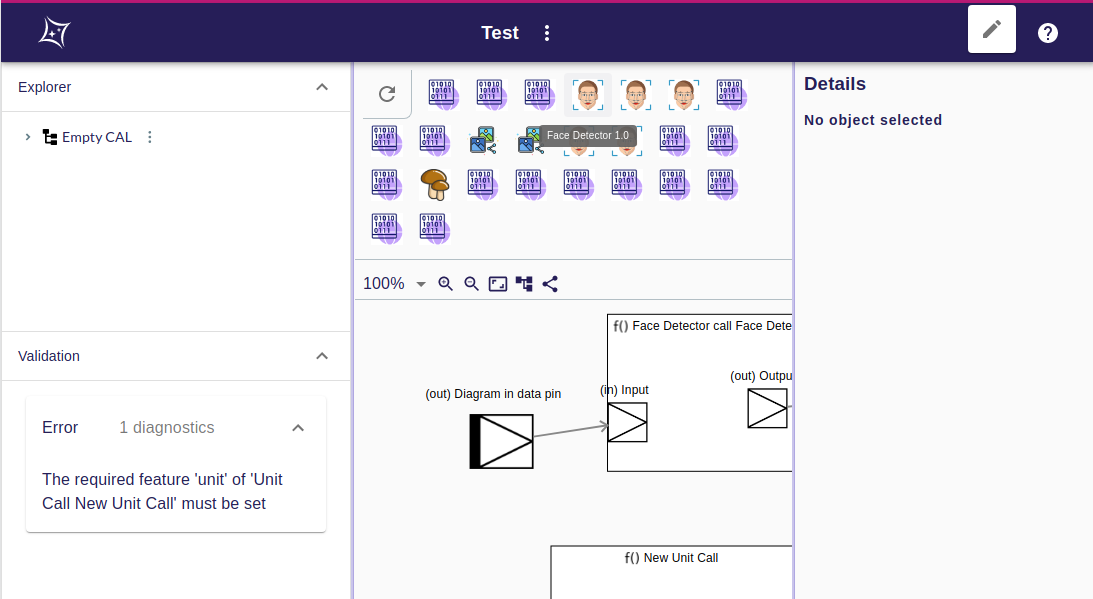
\includegraphics[width=0.95\linewidth]{./images/sirius-web-toolbox.png}
	\caption{Przybornik dodany w \emph{Sirius
			Web}.}\label{rys:sirius-web-toolbox}
\end{figure}

\subsection{Dodanie wywołania modułu obliczeniowego do modelu}

% Opis problemu dodawania nowych \texttt{UnitCall} do diagramu --- trzeba
% zdefiniować \texttt{ComputationUnitRelease} w diagramie.
%
% Rozwiązanie (zaczerpnięte z edytora diagramów BalticLSC) --- przybornik
% (toolbox).
%
% Opis jak to zrobiono, od strony backendu jak i frontendu. Omówienie trudności w
% modyfikacji interfejsu użytkownika Sirius Web (trzeba było skopiować kod
% źródłowy niektórych komponentów z biblioteki \textit{Sirius Components} do kodu
% aplikacji Sirius Web, ponieważ komponenty te nie umożliwiały modyfikacji
% interfejsu i wstawiania do nich nowych elementów --- najlepiej dać zrzut ekranu
% co można było łatwo zmienić, a co wymagało skopiowania kodu).

\section{Walidacja semantyczna modelu}

Informacja o informacjach diagnostycznych udostępnianych domyślnie przez Sirius
Web.

Brak uruchamiania reguł semantycznych zdefiniowanych w
metamodelu~\ref{sec:reguly-walidacyjne-metamodel}.

Opis dodanego rozwiązania (własne klasy Javowe które zwracają listę informacji
diagnostycznych, oraz strumieniowanie ich do przeglądarki wykorzystując
istniejące rozwiązanie do walidacji).

\section{Użycie edytora Sirius Web w
  BalticLSC}\label{sec:uzycie-sirius-web-w-balcitlsc}

Omówienie przygotowanego planu integracji.
